\chapter{Introduction}
% Introduce Galaxy Interaction, why is it important?
In the context of large scale structure of the universe, galaxies represent a fundamental building block of matter. Through cosmic time galaxies evolve \citep{2005Natur.435..629S}, this evolution leading to the local universe as we see it today. A key part galaxy evolution is that of mutual interactions between them. Mutual interaction has a number of influences on galaxies, from morphological distortion, to mass transfer, to increases in star formation, to merging where the two (or more) galaxies coalesce into a single system. Our best cosmological model, $\Lambda$-Cold Dark Matter, dictates that matter - ergo, galaxies - assembled hierarchically \citep{1978MNRAS.183..341W, 1991ApJ...379...52W}. Therefore, we must understand the effects of mutual interaction to not just understand galaxy evolution but to better understand our theories of cosmology.

We have come to understand that interaction has multiple impacts on the evolution of galaxies. The first, and most obvious effect, is that it leads to the distortion of the disks involved and the formation of dinstinct tidal features. Since the existence of such features being related to interaction was hypothesised to proved \citep{Toomre_72} they are the best morphological indication that two galaxies are interacting. Often, we attempt to only classify interacting galaxies from their morphology. To truly know if two or more systems are interacting, we require redshift information to ascertain their 3D distances from each other. However, spectroscopic information across the many million close galaxy pairs we know about is limited.

Mutual interaction has further effects on galaxies than simply morphological disturbance, although these remain poorly understood. It is widely debated about the role of interaction in nuclear ignition and enhancement in star formation of each system. While the former may not happen at all, the latter is generally accepted to occur while the specific strength and impact on the system remains highly debated. If such processes occur strongly, they can completely change the system that we are observing. Interaction has also been proved to have an impact on the gas reserves in a galaxy, often leading to the complete quenching of the system post-interaction. However, interaction has also been shown to rejuvenate the galaxies involved, and bring them out of a quenched state and into a star forming state. This is highly dependent on the specifics of the interaction. Finally, the role of environment in galaxy interaction is also a highly researched area.

The primary focus of this thesis is on the role of tidal distortion in formation of tidal features for the purposes of system identification and constraint. However, in this process, we must also keep an account of the other underlying processes occuring during interaction. Fully understanding them, and modelling them if necessary, is key to accurately inferring and linking galactic parameters to physical processes. The list of unresolved questions about galaxy interaction is long and complex. The focus of this thesis is in providing the tools to understand galaxy interaction and answer some of the fundamental questions regarding it. These questions include:

\begin{itemize}
	\item What do we require to improve our understanding of interaction?
	\item How do we better identify interacting galaxies?
	\item What is the relationship between numerous galactic processes and galactic parameters?
	\item From existing samples and studies, how do we better constrain our understanding on the effects of interaction?
\end{itemize}

To fully answer these questions about galaxy interaction, we require three things: first, the tools to find and create large statistically significant samples of interacting galaxies; second, available ancillary data of these systems to make inferences between the underlying processes in interaction and their parameters; and thirdly, the tools to betteer constrain these relationships. In this thesis, detail two pipelines which achive these goals. First,  In chapter 2, I will describe a pipeline for creating the largest interacting galaxy catalogue to date from combining morphological classification with novel methods of data extraction and analysis. I will then use this catalogue, in chapter 3, with cross matches to existing ancillary catalogues and make my own inferences about the relationship between galactic parameters and underlying processes. However, this will also show the limitations of only using observations and the requirements for constraint by simulations. Finally, in chapter 5,  I describe a pipeline that will conduct such constraint in the context of Bayesian statistics and galactic parameterisation. I will describe the results we have found by applying it to a small, well constrained, interacting galaxy sample and then describe the limitations of the approach in terms of computational efficiency. However, for now, it would be prudent to begin this discussion by exploring the definition of  a galaxy, and outlining the major work already conducted into linking galaxy interaction with galaxy evolution.

\section{WHAT IS A GALAXY?}
\noindent For the purposes of this work, a galaxy will be the smallest unit of mass we will be considering. A galaxy is an extended system of stars, gas and dust which all orbits around a supermassive black hole at its centre. All of this baryonic matter makes up the luminous, or visible, matter of the galaxy. This matter has two distinct components: the galactic bulge and the galactic disk. The galactic bulge lies at the centre of the system. It is an approximately spherical component which extends, typically, out to about a third of the radius of the galaxy. Galaxies will always have a bulge component, although it might be so small that the galaxy appears to only have a disk. The bulge is often made of an older population of stars, with high peculiar motions in their orbit. At the centre of the bulge, we find the supermassive black hole which, we believe, always resides at the centre of a galaxy. Often, this supermassive black hole is quiescent and simply existing at the centre of the galaxy. However, under certain circumstances we are still attempting to understand, the black hole can start accreting lots of gas. Whether driven by galaxy mergers \citep{} or secular processes \citep{}, the result of this black hole feeding and growth can cause an ignition of so-called nuclear activity. This is when the black hole begins to spew out lots of material perpendicular to the galaxy. When this occurs, we call it an active galactic nucleus or an AGN. About the the supermassive black hole and galactic bulge lies the galactic disk. The galactic disk is a very thin, extended region orbiting about these central components. This is where the majority of the galaxy's gas and dust reside. There are many younger stars throughout it as well, and this extends out to a radii many times that of the galactic bulge. Both of these are embedded in a dark matter halo.

The dark matter halo is many times the radius of the luminous components of the galaxy. This halo is also many times the mass of baryonic components of the galaxy, and makes up the majority of the mass of a galaxy. We approximate each of these components with different potential models. For the galactic bulge, we utilise a Plummer sphere \citep{1911MNRAS..71..460P}. For the galactic disk, we use an exponential disk model. For the dark matter halo, we utilise a cored Navarro-Frenk-White model \citep{1997ApJ...490..493N}.

For much of the history of extragalactic astrophysics, the idea that galaxies could interact and merge was thought to be very inprobable. The small radii of the luminous matter in galaxies, and their calculated cross sections, led astronomers to believe that the probability of an interaction was close to 0 and that galaxies were, simply, island universes  \citep{1926ApJ....64..321H}. However, with the development of the idea of the dark matter halo, with its radius many times that of the luminous matter, it was realised that the probability of galactic systems interacting and merging was within the realm of possibility. And, therefore, over time the idea that galaxy interaction and merging would have a significant impact on galaxy evolution was developed. In fact, the merger rates of galaxies through cosmic time is one of the most well studied concepts of our cosmological models with observations and simulations.

\section{GALAXY ASSEMBLY ACROSS COSMOLOGICAL TIME}
\noindent Galaxies, throughout cosmic history have been assembling and accreting matter to form the universe that we see today. Studies at high redshifts reveal that gaalxy structure is significantly different when compared to today. Initially, galaxies were very small systems that formed from gravitational instability thoughout the early cosmos \citep{1993MNRAS.262..627L}. These instabilities were generated by the physical processes of the very early universe brought about by the small scale of the universe. From these initial density perturbations arose small systems which accreted from the gas and dust throughout the early universe. These early galactic systems were much smaller than those we see today. Their morphology was also very peculiar, and they were forming stars at a much higher rate than galaxies in the local universe. While these systems were accreting much of their matter to gain mass, the universe was expanding. At this time, with the universe at a much smaller scale, the rate of galaxies interacting and merging was much higher than today \citep{2010ApJ...715..202H, 2011ApJ...742..103L}. This provided a peak in the cosmic star formation of the history through 1 $<$ z $<$ 3 where approximately half of all stellar mass was formed \citep{2005ApJ...625..621B}.

Figure \ref{fig:merger-rate} shows the changing merger rate through cosmic time. As the merger rate increased, peaked and then declined it had profound effects on both the star formation density of the universe and the morphology of those galaxies within it. From z = 1, the once massive galaxies, with rapid star formation, have transformed into bulge-dominated galaxies contraining super massive black holes \citep{2007ApJ...654..858B}. In fact, as we go to lower redshifts, we find that the majority of the stellar mass is contained within these systems. These galaxies are dominated by old stellar components and have little ongoing star formation \citep{2002AJ....124..646H, 2004ApJ...608..752B}. Thus, showing that mergers were the primary drivers of star formation in the past. 

\begin{figure}
    \centering
    \includegraphics[width=0.95\textwidth]{Introduction/figures/merger-rates.png}
    \caption{The clearly declining merger rates from z = 3 to z = 0. This is Figure 3 of \citet{2010ApJ...715..202H}. This study looked at the history of a simulated set of galaxies of various stellar mass, and investigated the decrease in the merger fraction as a function of redshift and baryonic mass. As shown, for all mass bins and methods of identifying mergers (the different lines) the merger rate decreases. This is only not true for mergers between very high mass systems and low mass systems (in the bottom right of this plot). Thus, mergers between high and low mass systems may still have some driving force in the cosmic star formation rate density.}
    \label{fig:merger-rate}
\end{figure}

%\begin{figure}
%    \centering
%    \includegraphics[width=0.95\textwidth]{Introduction/figures/}
%    \caption{}
%    \label{fig:example-of-code}
%\end{figure}

The morphology we see now, that formed out of this period of very intense merging and interaction, was first offically defined in \citet{1936rene.book.....H}. The famous `Hubble tuning fork', was once thought of as a map of galaxy evolution, is now known to be one of galaxy morphological classification. Figure \ref{fig:hubble-tuning} shows this breakdown of morphological classification, from spheroidal systems on the left to disky spiral or disky barred galaxies shown on the right. What was once thought of as a layout of galaxies with age, we now understand as an indication of the evolutionary history of individual systems. From our description here of merger rates, we realise that the systems on the left of the tuning fork are actually those with intense merger histories and that are far older than those on the right. These are spheroidal systems, also called early-type galaxies contain little gas, have almost no star formation and appear very red in our colour-colour charts. Those systems on the right are slightly younger than the early-type systems but have a less intense merger history, especially in the last few Gyrs \citep{}. While they could have This leads them to with plentiful gas, lots of star formation and a blue appearence.

\begin{figure}
    \centering
    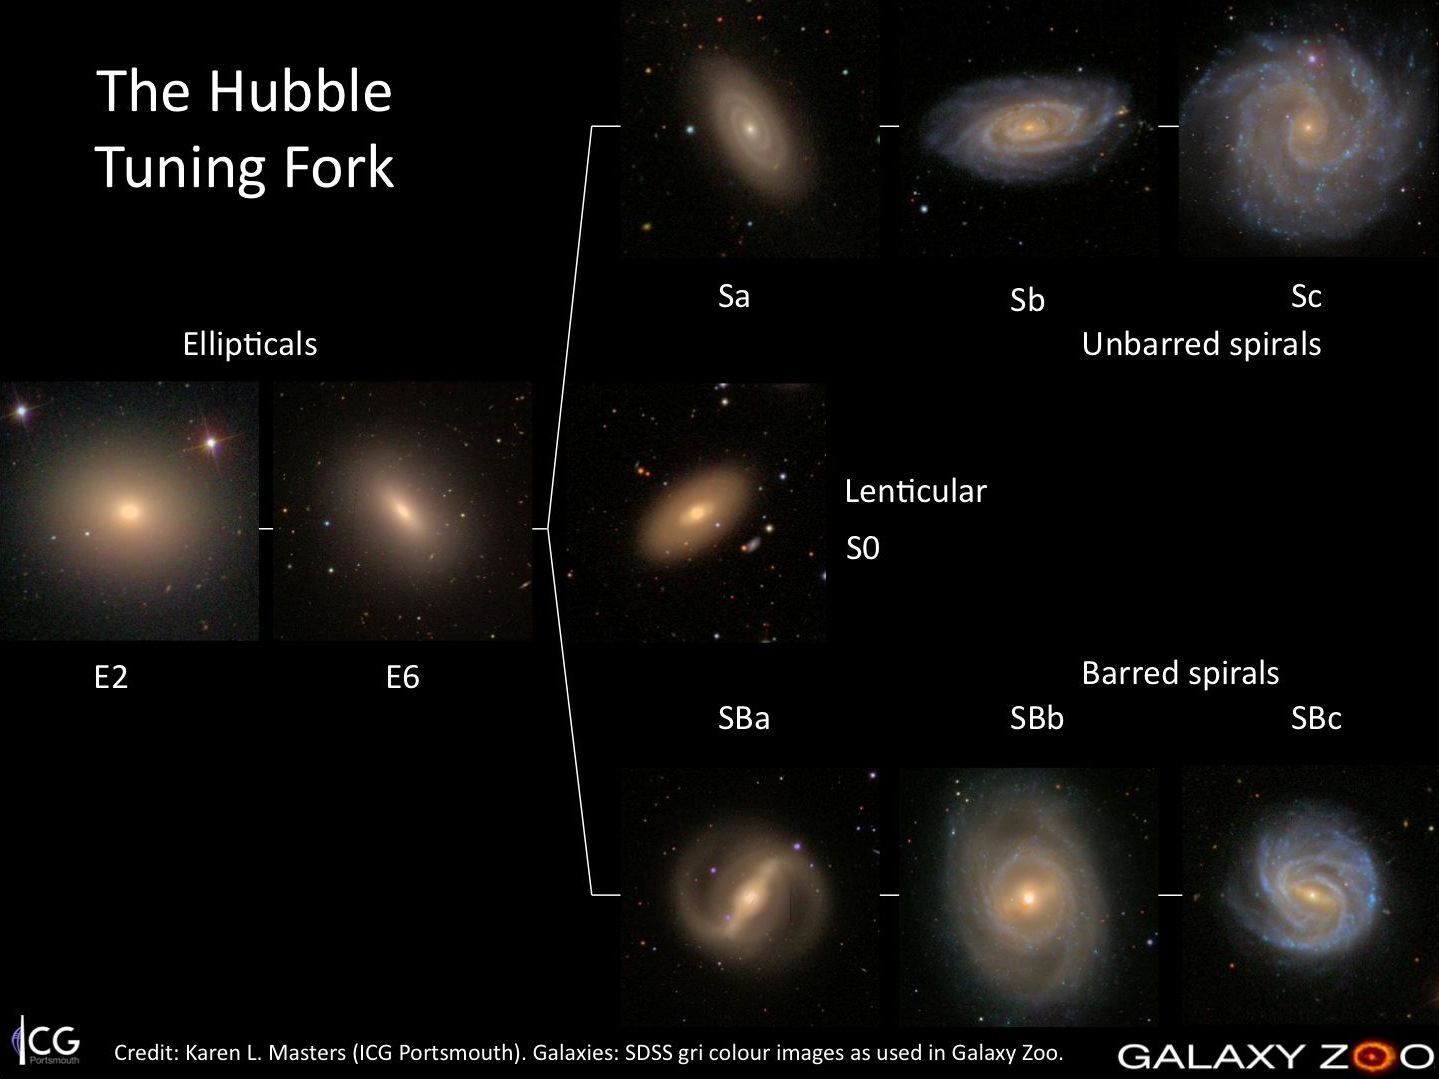
\includegraphics[width=0.95\textwidth]{Introduction/figures/hubble-tuning-fork.jpg}
    \caption{The Hubble tuning fork. Credit goes to the Galaxy Zoo collaboration (and specifically Karen Masters) for the creation of this figure. What was once thought of as an evolutionary track for galaxies, is now a widely adopted classification system for them based on morphology. On the left, we have elliptical systems - so called early-type galaxies - which are often `red and dead' systems. They have an intense merger history, which has destroyed their disk component and caused them to use the majority of their gas in star formation. On the right, we have two different kinds of disk galaxies. Ignoring the bar or un-barred part of this, they are systems which have a less intense merger history and have only accreted smaller systems into them. This serves to enhance their gas disk, and preserve their disk component.}
    \label{fig:hubble-tuning}
\end{figure}

Thus, as the merger rate has decreased through cosmic time, the survival of disk galaxies has increased. We, therefore, see two dinstinct populations of galaxies which can be easily defined by their morphology and colour which directly relates to their own evolutionary and merger history. One is of galaxies with a history of intense interactions with galaxies of equivilent mass, which lead to the complete destruction of their disks, and the other is of galaxies with a less intense merger history, with systems of much smaller mass than their own. These interactions and mergers serve to feed the gas within the galactic disks and increase their mass, while preserving the disk component of the system. In this thesis, I will not focus on merger rates any further than already explored. However, this whole discussion feeds into how we best identify mergers and interacting galaxies. I will, therefore, briefly discuss the morphology of galaxies and how it links into their properties. This will put things into perspective before I discuss how these systems are completely disrupted by merging and interaction. 

\section{GALAXY MORPHOLOGY \& GALACTIC PROPERTIES}
\noindent Galaxy morphology, and its change with time, specifically is the study and measure of a galaxies shape and features so that we can make different assumptions about it. There are many examples of morphological studies of galaxies. One of the largest to date was that of the Galaxy Zoo collaboration first published in \citet{2008MNRAS.389.1179L}. This project created the colour cutouts of $\approx$900,000 galaxies and presented them to citizen scientists for visual inspection. A citizen scientist is a volunteer who wishes to partake in answering scientific questions or annotating data in their spare time. Classifying nearly a million images by an individual is nearly impossible to do with any reasonable efficiency. However, in this project, nearly 100,000 volunteers stepped up to the task. Thus, each cutout could be visually inspected by different individuals who could make their own decision on the morphology of the galaxy. If enough individuals made a classification, one can then minimise the uncertainty in those classifications and find the answer from a group rather than leaving it up to an individuals opinion. Originally, this project made 40 million classifications across a range of morphologies. In the present day this collaboration has made hundreds of millions of classifications across a range of telescopes, redshifts and different morphology types.

The most important question asked in this - concerning morphology - is if the galaxy is smooth or a disk. As stated previously, this immediately gives an indication of multiple galaxy properties. First, if a galaxy is elliptical, it is likely that it is much redder than a disk galaxy \citep{1992MNRAS.254..589B}. Elliptical galaxies are dominated by their bulge component, meaning they are highly dispersion dominated and spheroidal in shape. As stated previously, this indicates a turbulent merger history, that has destroyed the ordered rotationally dominated component of a galactic disk. As a result of this, the gas mass and density are very low, having been removed by internal or external processes \citep{1976ApJ...204..365F}. As a result, the rate of star formation (or, more colloqually, the star formation rate; SFR) within these systems is very low - particularily when compared to disk galaxies. The gas within the galaxy has no opportunity to condense, fragment and form stars as required.

This low gas mass and low SFR within these galaxies has direct effects on their observable. The stellar populations that make up these galaxies are older and, therefore, lack the high mass and luminous OB-type stars that are typical of star forming regions. These stars are short-lived (only about a few hundred million years) and go supernova quickly in the history of these galaxies. The remaining smaller mass stars dominate the spectral energy distributions we observe of these systems. We can observe different parts of these distributions by using different filters on our telescopes. This leads us to defining a galaxies colour: the difference between the measured magnitude of flux in two different filters. Elliptical masses are often found to be red, in this system. We define red, in this context, as the difference between the `green' filter and the `red' filter (centered on 4,770$\AA$ and 6,231$\AA$ respectively). The green filter is designed to capture the part of the SED which is primarily contributed to by young or main sequence stars while the red captures that part from older, smaller mass stars \citep{Part of the SED we observe in each filter?}. Thus, when we subtract the magnitude observed in each filter, g-r, if this is very small we have a red galaxy and if it is very large we have a highly star forming galaxy. 

% Talk about the blue-ness of disk galaxies.
The opposite is true for galaxies which are primarily a disk. As stated previously, these systems have had a less tumultous merger history - particularily since z $\approx$ 1. An indicator of the merger or interaction history in disk galaxies is, in fact, the size and shape of the bulge component \citep{Bulge component is an indicator of merger history}. However, because of the plentiful gas, dust and ordered rotation in the galactic disk the SFR within is larger than elliptical galaxies. Gas clouds can condense and form throughout the galactic disk. It is well known that the surface density of molecular gas is directly related to the SFR throughout the galaxy \citep{Citing kennicutt, Schmidt etc}. Thus, the galactic disk provides the perfect environment for star formation. Spiral arms can exist in such galaxies, containing large filaments of gas and dust. They contain areas where large molecular clouds can condence, fragment and then collapse into new stars. These star forming regions will be young enough that massive OB-type stars will form, and be detectable to us. This increases the flux and magnitude found in the g band in our above equation. Thus, disk galaxies are often called `blue' galaxies, as the green value is much larger than the red in our colour observations.

\begin{figure}
    \centering
    \includegraphics[width=0.95\textwidth]{Introduction/figures/population-distribution.png}
    \caption{The distribution of galaxies in colour-colour space showing two distinct populations in a clear bi-modal structure. This is using the u-band and r-band filters and, therefore, the closer to 0 on the y-axis the bluer the galaxy. Left plot: the top population is the blue cloud, primarily composed of disk galaxies with young, star forming stellar populations. The bottom population is the red sequence, primarily composed of more massive elliptical galaxies which are gas poor and quiescent. Between these two populations lies the green valley, marked by the green lines. This is believed to be a transitional population moving between the blue cloud and red sequence for debatable reasons. To further show the split with morphology, the panels on the right split the colour-mass space into early-type (elliptical) galaxies and late-type (disk) galaxies. Note, this is Figure 2 of \citet{2014MNRAS.440..889S}}
    \label{fig:blue-red-population}
\end{figure}

% Now, talk about the blue and red sequence.
This gives rise to two distinct populations of galaxies: old, red elliptical galaxies and young, blue disk galaxies. When plotting colour-colour or colour-magnitude diagrams, these two populations are very clearly distinct with the `green valley' running between them. Figure \ref{fig:blue-red-population} shows the colour-colour distribution if the two populations. In this Figure, we clearly can see the blue population - blue cloud - and the red population - red sequance - beneath it with the green valley in between. The green valley is a disputed area of this distribution. Some works claim that it is a transition phase \citep{Papers green valley stuff. Start with Becky's work.}, where galaxies are moving between the two populations due to different processes, while others dispute this, and claim it is either a result of selection effects \citep{I think this is the red herring paper} or a different classification of object entirely \citep{Or this is the red herring paper}. However, what is definitive is that the rule of red galaxies are elliptical and blue galaxies are disk galaxies is not ubiquitous \citep{2022MNRAS.510.4126S}. Examples of blue ellipticals and red spirals do exist \citep{2022AJ....163..150K} and they are the subject of intense debate and study in the current field. However, as a general guideline for the expected properties of a galaxy the colour and morphology are deeply interdependent on one another.

% Want to introduce the idea of starburst galaxies, remnants and such here.
There are also many types of systems that do not fit this simple morphological definition of galaxies. Galaxies defined as starburst galaxies are often very morphologically irregular and have measured g-band fluxes, and therefore SFRs, far in excess of expectation for their mass. These then lead into post-starburst galaxies and merger remnants, who are the complete opposite and have very high measured r-band fluxes and therefore much lower SFRs. These are often called quiescent galaxies. These highly irregular systems have direct interplay, however, with their merger histories \citep{paper on post-starburst galaxies and merger remnants} and surrounding environments \citep{Paper on post-starburst galaxies and environment}. In fact, it has been found that in cluster environments, the fraction of disk galaxies drops to $\leq$10\% when compared to $\approx$60\% in the field.

The effect of the galactic environment on a galaxy should also not be understated. There are many ways to define the galactic environment, but it is most commonly associated with the number density of galaxies about them \citep{galaxy environment paper}. There are three broad classifications of environment: field, filament and cluster. A field galaxy is one with neighbours, and is in relative isolation. A filament galaxy has some neighbours, but their influence on the galaxy in question is minimal. A cluster galaxy is one in which a large number of other galaxies are bound in colossal galaxy cluster structures. In these environments, SFRs are suppressed \citep{Paper on environmental suppression} by ram pressure stripping and galaxy morphology is highly irregular due to constant interaction and merging. In these environments, the relation between galaxy morphology and the underlying processes is almost completely broken by interference from the environment.

Thus, galaxies in the field or in filaments are of particular interest. Here, we can study the direct link between morphology and the underlying processes of galaxies. And these, in turn, are highly dependent on galaxies underlying merger and interaction histories. So, what is this relation? As stated previously, the influence of interaction and merging accelerates the evolution of rotational systems to dispersion dominated systems. However, there are many more subtle affects that can be attributed to galactic merging and interaction. For instance, if two galaxies can be brought into a state of starbursting due to merging \citep{Paper on starbursting galaxies in interaction.}. This completely changes the underlying SED of the galaxies involved, and can lead to the rapid quenching both systems \citep{Paper on quenching a galaxy with interaction}. Thus, depending on when we observe such a galaxy, we can find either a much bluer or redder galaxy than expected. However, it can also be found that such interactions do not lead to much change in the underlying SED at all \citep{Paper on not much change in the SED of a galaxy}. So, why is this? It transpires that the effects of a galaxy merger or galaxy interaction are dependent on the underlying parameters of the galaxies themselves. This leads to us having multiple classifications of galaxy interactions which each lead to different outcomes for the galaxies involved. 

\section{CATEGORISATION OF MERGERS}
\noindent The effects of galaxy interaction and merging is dependent on multiple different factors and underlying parameters. However, the two most important parameters are the mass ratio \citep{paper saying mass ratio is important} and gas content \citep{paper that says the gas content is important} of the galaxies involved. The impact parameter also does have a lot of influence over the final morphology over the system, however, we will discuss this further in the next section. The recognition that the mass ratio and the gas content of interacting galaxies leads to significant outcomes means that a small categorisation system has been produced to recognise the different kinds. For the mass ratio, we define a major, a minor and a micro interaction \citep{Paper with these definitions in them?}. These are the ratios of the primary galaxy mass (the more massive galaxy) and the secondary galaxy mass (less massive galaxy). These are then further sub-divided into two seperate categories based on their gas content: a wet merger or a dry merger \citep{Paper on wet vs dry mergers}. This refers to the gas mass and colour of both galaxies. A wet merger involves lots of gas in the two galaxies colliding, and therefore, lots of resultant star formation. Both of the involved galaxies are blue, and often disk-dominated galaxies. A dry merger involves little gas, and is often the merger of massive, red elliptical galaxies. There are also intermediate categorisations based on the amount of gas, such as damp mergers (where there is some gas, but not enough to completely dramatically increase star formation) and mixed mergers (mergers between gas-poor and gas rich systems) \citep{Paper on mixed / damp mergers}, however, we focus on the binary definition of wet and dry mergers.

Depending on the classification of an interaction leads to specific outcomes for the interacting galaxy system. A major interaction is when the galaxies involved have a mass ratio of approximately 1:1. Some definitions vary, however, and allow this limit to go down to 1:3. For the purposes of this work, they must have a mass ratio of approximately 1:1. Major interactions are the most devastating to the morphology of the systems involved, with the forces upon them causing severe morphological distortion and the formation of tidal features (more on this in the following section). If the two systems merge, there is complete destruction of the disks in both galaxies and the post-merger remnant will be highly irregular. If this major interaction is also a wet one we would also expect a significant increase in the SFRs of both galaxies \citep{Increases in SFR in wet interactions} - this is particularily true if the two systems actually coalesce \citep{Papers on increases in SFR in coalesced mergers}. We also find that wet major mergers have an increased AGN fraction \citep{Paper on wet major mergers and AGN}, which suggests that such a merger may play a role in nuclear ignition. The opposite of this is true when a major interaction is dry, where only a small increase in SFR is found in the nuclear region of the galaxies \citep{Papers on dry mergers leading to increased SFR in the nuclear region}. This holds true even when the two systems actually merge, with no significant change in SFR or AGN fraction emerging at all.

\begin{figure}
    \centering
    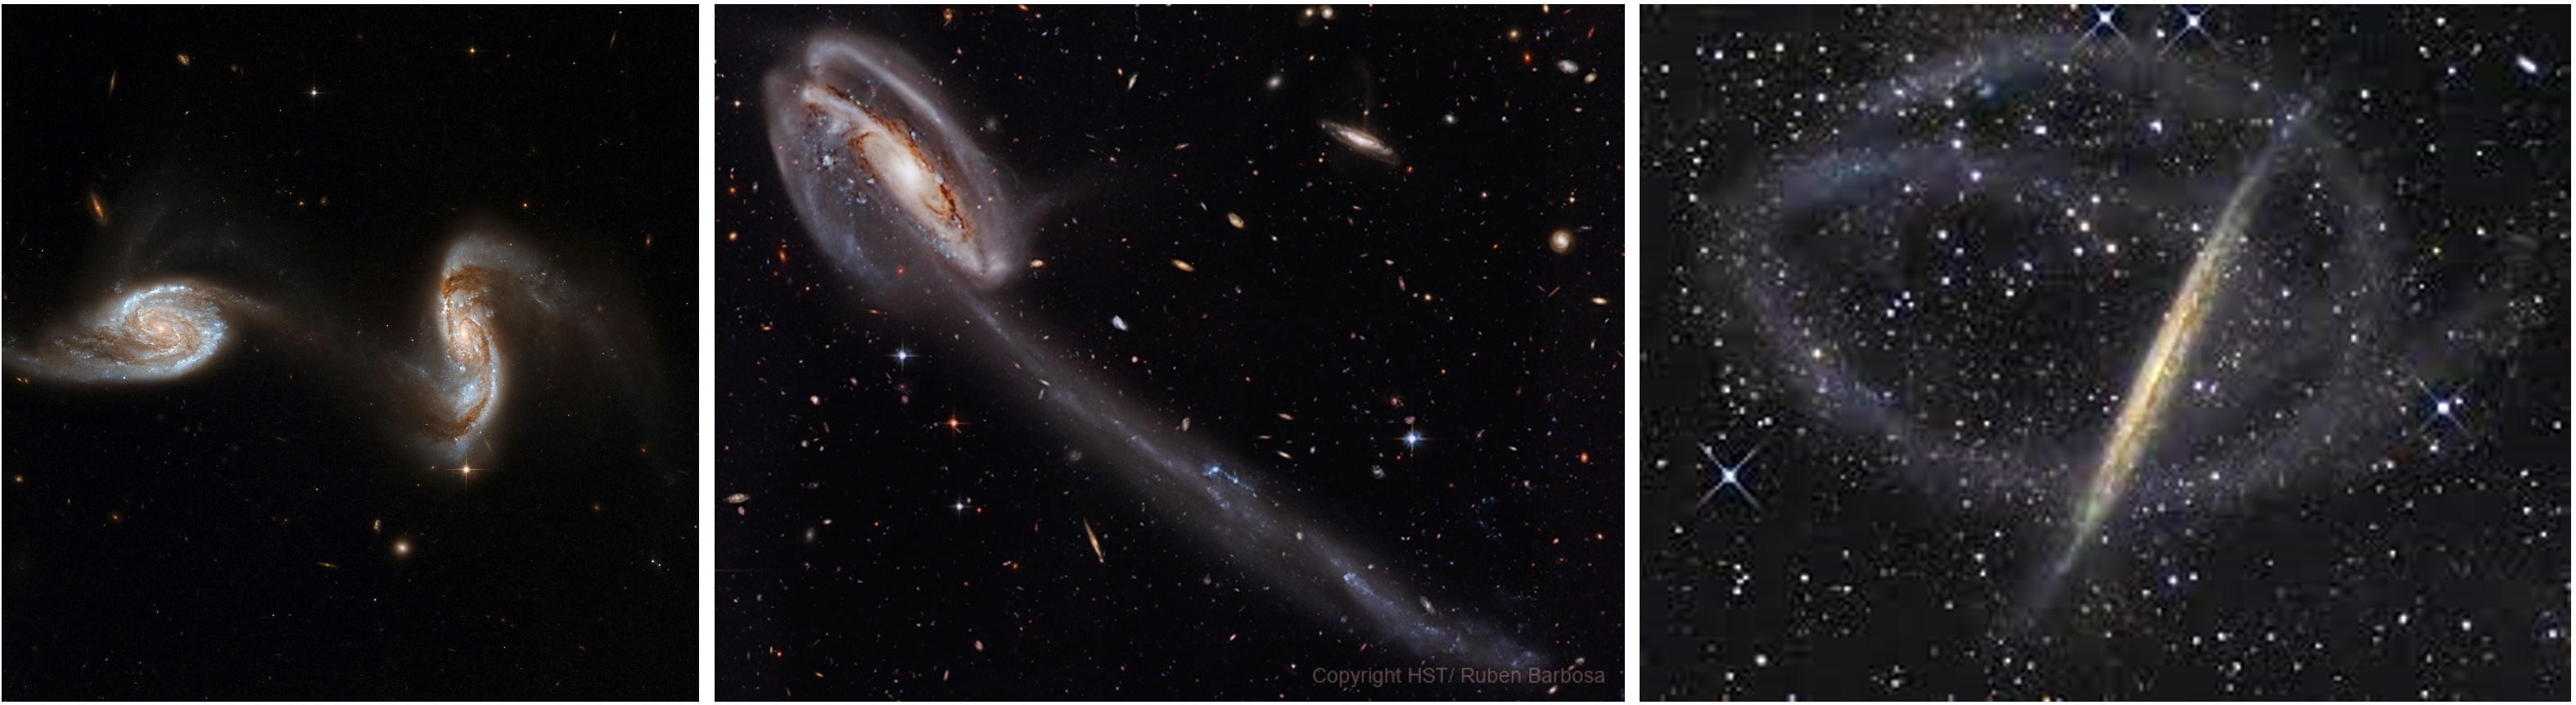
\includegraphics[width=0.95\textwidth]{Introduction/figures/combined-examples-mergers.jpg}
    \caption{Examples of a major, a minor and a micro interaction. Each of these are wet interactions, containing lots of gas and therefore increases in star formation. These are the Arp 240, Arp1 188 and NGC 5907 systems, respectively. Here, we show the famous double looped stellar stream of NGC 5907 but point out that the existence of the second loop is in dispute and that we only show it here for illustrative purposes. From major to micro interactions, we see decreasing impact and change in the morphology of the primary galaxies but always the complete destruction of the secondary.}
    \label{fig:merger-clsfs}
\end{figure}

A minor interaction has less catastrophic consequences for the morphology of one of the two galaxies. This is defined as an interaction where the mass ratio is less than 1:1 but greater than 1:10. Due to this large mass disparity, the morphology of the primary galaxy is relatively unaffected by such an interaction. However, the secondary galaxy will be almost completely destroyed by the encounter. If it is only flying by in an interaction, the secondary will be higly disrupted, forming a long and stretched tidal tail as it moves through the orbit. This will leave a large stellar stream around the primary galaxies disk, which can become a probe of the dark matter halo about the galaxy. In a wet merger, the tidal tails formed in the secondary galaxies can often condense into their own tidal dwarf galaxies \citep{Papers on tidal dwarfs}. This leads to interesting, dark matter-less systems that we can explore and test alternative theories of cosmology \citep{Papers on MOND and that sort of thing}. When these systems actually merge, we observe small increases in the SFR of the primary. There is ongoing work investigating whether such mergers were actually a primary driver of star formation in galaxies across cosmic time \citep{Sugata's paper on the work} with contradicting results \citep{Papers with minor interactions being primary drivers of cosmic SFR}.

Finally, a minor interaction is one in which the mass ratio between the primary and secondary galaxies is less than 1:10. This always sees the complete destruction of the secondary galaxy, whether just a flyby or a complete merger. A very local example of this is the interaction of the satellite galaxies of the Large and Small Magellanic Clouds \citep{Papers that say the LMC and SMC are examples of micro mergers}. These also form many stellar streams about their primary galaxy and are often absorbed by the primary with very little change in its morphology. Therefore, it has been theorised that such mergers could be a much larger driver of cosmic star formation through time but leaving very little evidence or impact on the primary galaxy. 

Figure \ref{fig:merger-clsfs} show examples of each of the different merger categories we have defined here. These, from left to right, are the Arp 240, Arp 188 and NGC 5907 systems. They each show a major, minor and micro interaction, respectively, and demonstrate the change in effect the mass ratio has on the morphology of the galaxies involved. From Arp 240, with the complete destruction of the galactic disks and formation of tidal features to NGC 5907 where the primary galaxy is barely disturbed at all. Thus, the different categories of interactions and mergers have very different impacts on the systems involved. I will now discuss, in depth, the effects that interaction has on these galaxies and specifically explore the formation of morphological disturbances like tidal features, changes in the SFR and the increase in AGN fraction.

\section{EFFECTS OF GALAXY INTERACTION}
% Here, present examples of interacting galaxies and the context in which we're talking about them.
The idea of two or more galaxies interacting and the effect that it would have had upon galaxy formation and evolution was thought to be minute \citep{Found this info in Chapter 8 of Binnie and Tremaine. Need to find a better source!}. We now understand that galaxy interaction plays an important, and fundamental role in the evolution of galaxies. As stated previously, they have multiple affects upon the systems undergoing the interaction. The specific effects of interaction lies on a host of parameters, we have discussed the mass ratio and gas content and mentioned the impact parameter but there is also the orientation of the interaction, the relative sizes of the galaxies and the point in the dynamical history of the interaction we are observing \citep{Some review paper, perhaps that states that these parameters are important}. Thus, in this section, we will explore how these different underlying parameters link to the physical processes we observe in interacting and merging galaxies.

% For each of these sections below, I want to do a deep dive on how each process is driven. Will maybe mention simulations throughout, but we shall see?
\subsection{Morphological Distortion: Tidal Features}
% Introduction here: What do I mean by tidal distortion? What are we actually looking at?
\noindent It is important to start here with pointing out that galaxies are large gravitationally bound systems of stars, interstellar gas, dust and dark matter. Upon a close encounter between two galactic systems, these components experience strong gravitational forces which disrupt their ordered layout. AS the galaxies move rthrough their relative orbits, the gravitational potential changes at an accelerating rate. This imparts energy into the ordered components of the galaxies, and caused thermalization of their internal motions. This leads to violent relaxation, where the stellar orbits are so altered they no longer follow their prior orbits. However, the energy in the system must be conserved. Thus, as the internal stellar motions within the galaxy gets thermalized, the energy in the galaxy's orbits decay via dynamical friction. If this decay is large enough, the energy in the galaxy's orbit may be sufficiently reduced to no longer escape from one another and they will eventually coalesce to leave a single merger remnant. 

However, before this, the changing graviational fields as the two galaxies encounter each other leads to radial distortion of each galaxy. This leads to the drawing out of galactic material into long plumes which can eventually become tails. If stellar material, including gas, dust and stars, is close to the edge of the galaxy a combination of the galactic rotation and radial elongation lead to it being sheared off and away from the galaxy. This forms two `tidal tails` in the system, one leading and one proceding the motion of the galaxy. Dependent on the geometry of the encounter, the trailing tail of one galaxy and the preceding tail of the other can form a `tidal bridge' - a linking of the two systems. An example of both of these is the interacting pair Arp 240, shown in left hand plot of Figure \ref{fig:merger-clsfs}. 

The geometry of the bulk motion of the galaxy is very important in forming these tidal features. As the internal galaxy rotation and bulk motion in of the galaxy's orbit in the encounter must match for this shearing of material to occur. Thus, the formation of tidal tails and tidal bridges is only possible in a prograde interaction whereas a retrograde interaction suppresses them \citep{Papers on prograde and retrograde interactions}. Further, depending on the relative velocities in of the galaxies these tidal tails can be split off from the galaxy as the encounter continues. This can lead to the formation of `tidal debris' of stellar material forming about the galaxies. In some instances, this tidal debris can actually coalesce and form galactic systems of their own \citep{Papers on tidal dwarfs and need to actually proof this is a thing}.

While the most striking tidal features to form in galactic encounters are these tidal tails and bridges, we also see the formation of a slew of other features. These include `stellar streams' (previously discussed), shells and rings forming in the galactic disk. As stated, stellar streams are likely smaller galactic systems that have been destroyed while passing the primary galaxy. This leaves a faint stream of material about the galaxy. The right plot of Figure \ref{fig:merger-clsfs} shows an example of a stellar stream with the NGC 5907 system. Shells, on the other hand, are formed about galaxies and can be present in as many as 30\% - 50\% of elliptical and lenticular galaxies \citep{Shell presense in galaxies}. The left panel of Figure \ref{fig:tidal-features-ex} shows an example of shell in the elliptical galaxy NGC 1344. Spectroscopy shows that shells are primarily composed of stars. There are often numerous shells in a single galaxy, although most often we only detect $\approx$3. Shells are formed from the disruption of a small satellite around a significantly more massive galaxy - so, in a minor to micro interaction. This then forms a stellar stream, which overtime condenses to a cloud of stars orbiting the primary galaxy. This then either forms into an X-shaped structure or a annulus which, in the 2D projection of the sky, appears as a shell. Thus, observing a stellar stream or a shell is highly dependent on the time in the dynamical history of the encounter that we are observing.

\begin{figure}
    \centering
    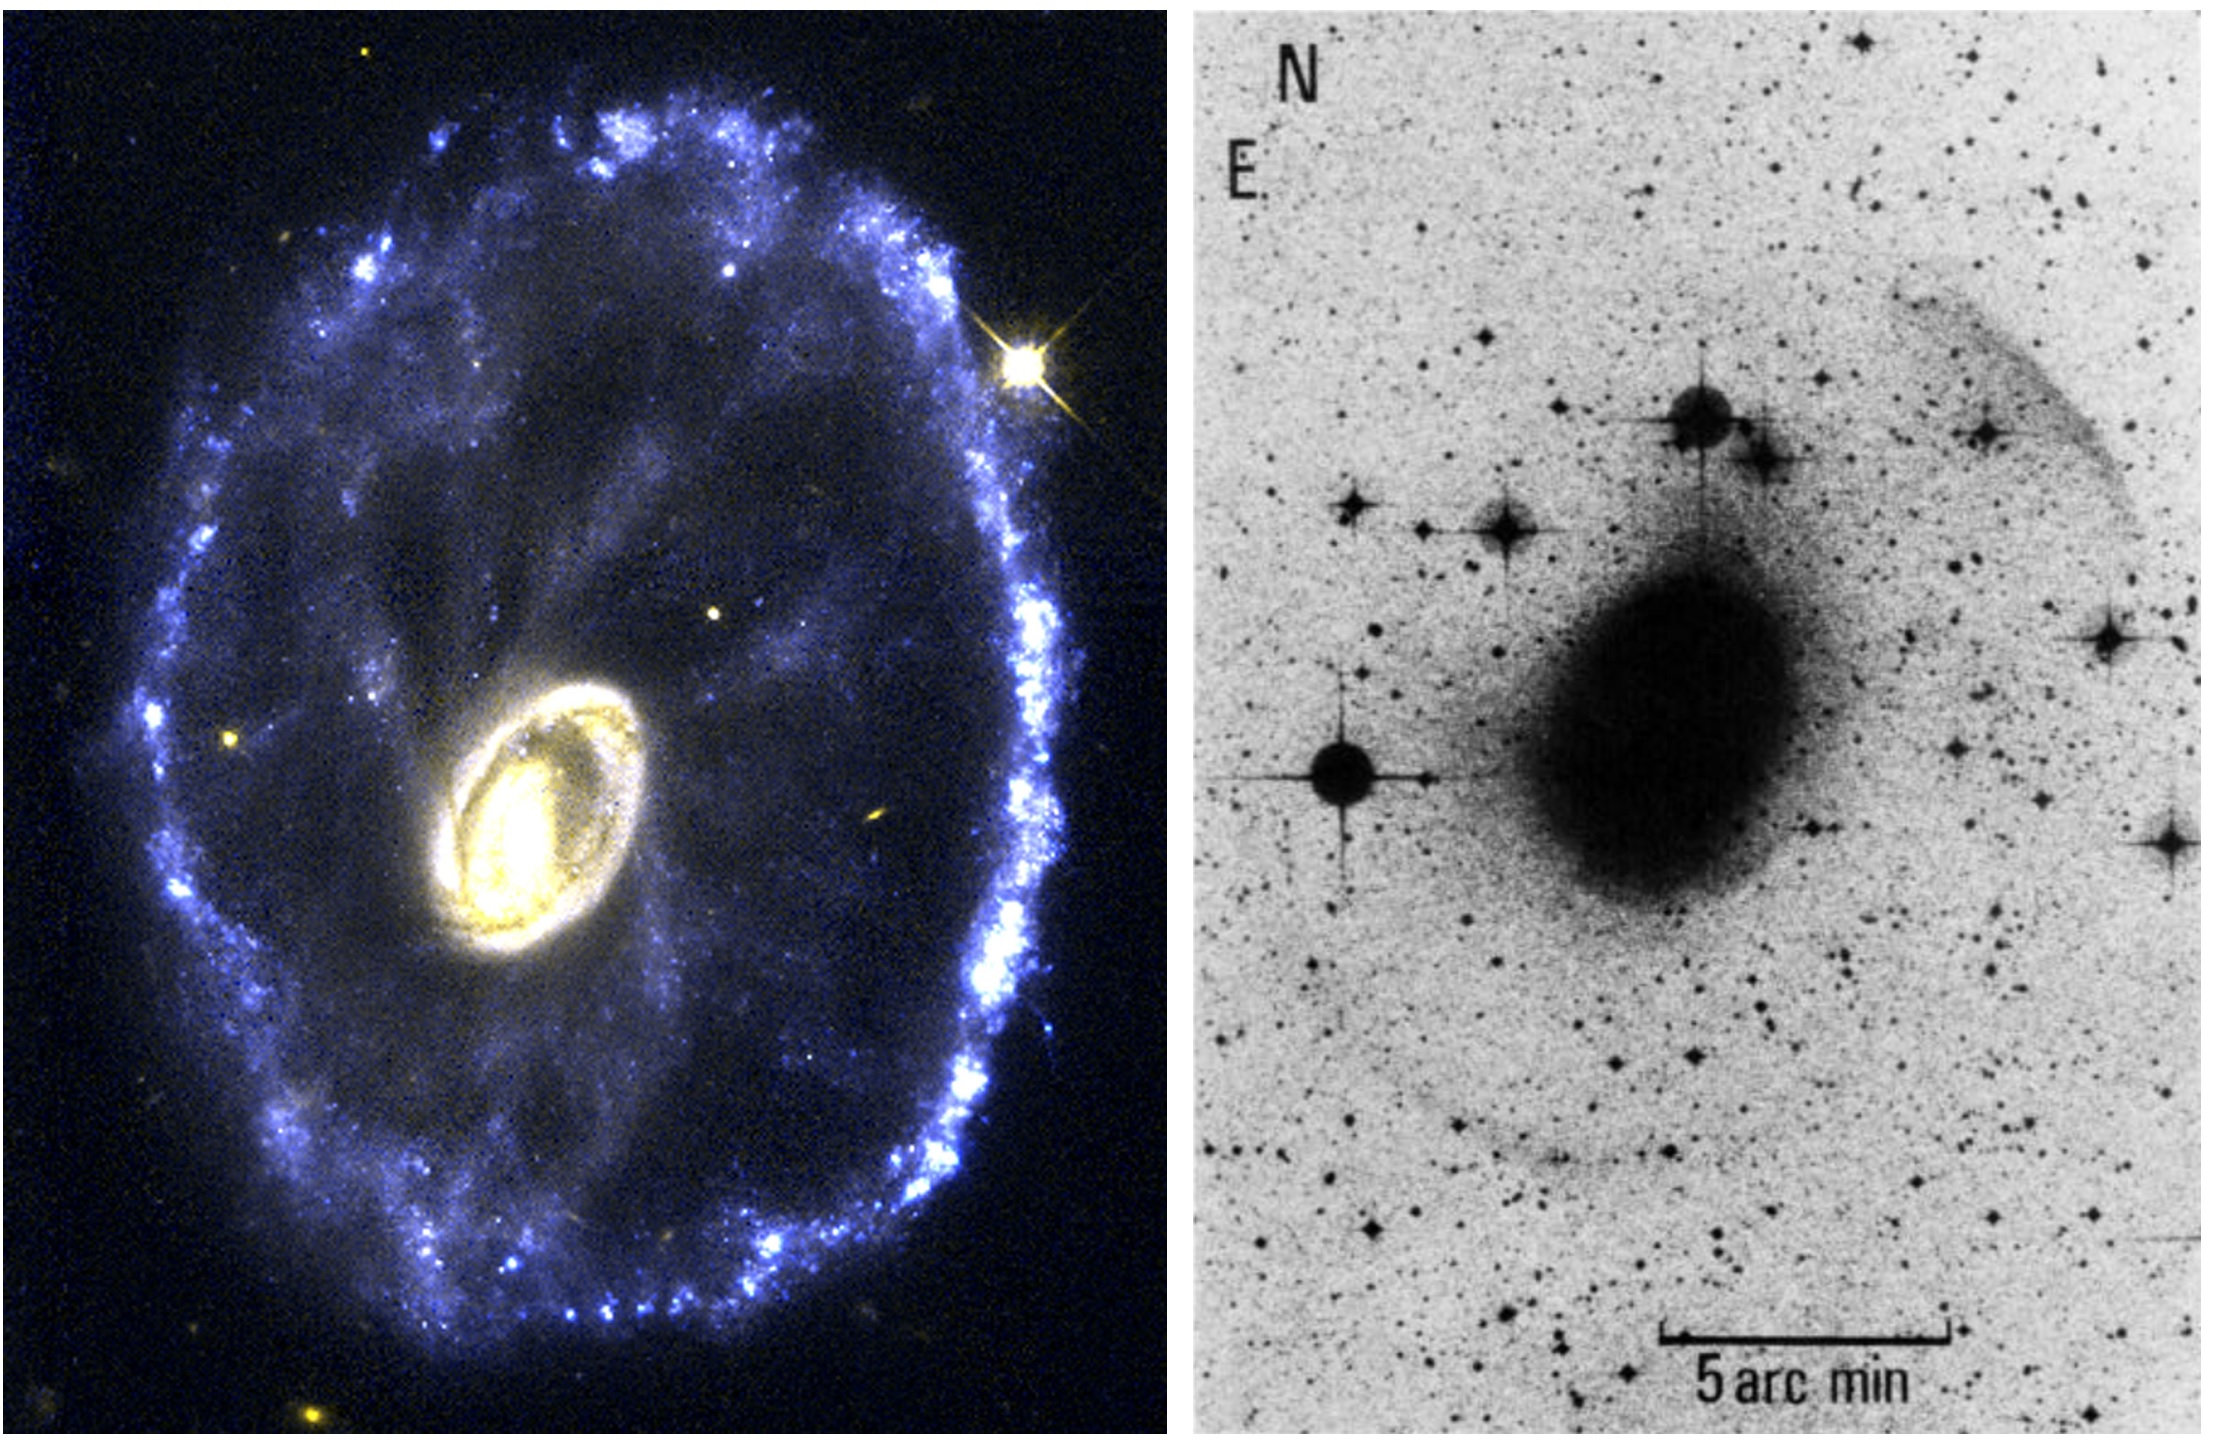
\includegraphics[width=0.95\textwidth]{Introduction/figures/shells-rings.jpg}
    \caption{Examples of a collisional ring galaxy and a system containing shells. Left: The Cartwheel galaxy, the most famous ring galaxy to date. Ring galaxies can only formed by a direct, head on collision between two galaxies. The ring itself is composed of a region of the disk undergoing intense star formation due to the density wave passing through the disk from the impact of the secondary galaxy. Right: The system NGC 1344, showing two shells of stellar material about it. This is formed by the condensation of stellar streams into clouds of stars. Cartwheel Galaxy Image: NASA / Hubble, NGC 1344 Image: \citet{1983ApJ...274..534M}}
    \label{fig:tidal-features-ex}
\end{figure}

Finally, we find rings can form from galaxy interaction. These systems are often called ring galaxies or collisional ring galaxies. Figure \ref{fig:tidal-features-ex}'s right panel shows the Cartwheel Galaxy: a famous example of a ring galaxy. This ring is formed of young, hot stars and is formed only from the head-on collision with another system \citep{Lynds and Toomre 1976}. The interaction to form this is so intense, that it causes a density wave to pass through the galactic disk which triggers intense star formation at its wake. These systems are incredibly rare, as this requires an impact parameter of 0 for this feature to form.

From the example of a ring galaxy, we see that interaction not only affects the stellar distribution of the galaxy, but also has direct impacts on the gas within it. As I have stated in previous sections, interaction and merging can induce enhancements in star formation and even lead to a starburst in a galaxy which brings about the complete quenching of the system.

\subsection{Star Formation Enhancement} 
\noindent As stated previously, it is often observed in interacting and merging galaxies that the star formation is enhanced in some way. While to what level this enhancement is often debated between observations \citep{} and simulations \citep{}, the underlying processes that lead to enhancement is well understood. First, by star formation enhancement we mean that the SFR either globally or in different regions of an interacting galaxy is higher when compared to isolated galaxies. Thus, some property of interaction is causing an increase in the star forming activity of the galaxies involved. 

The rate at which stars form is known to be directly related to the surface density of gas at any given piont within the galaxy. The global version of this idea is the Kennicutt-Schmidt Law \citep{Kennicutt-Schmidt paper} and finds a tight correlation between these two parameters like so:
\begin{equation}
	\Sigma_{SFR} \propto \Sigma_{Gas}^{n}
\end{equation}
where n = N. Thus, this applies to within the galaxy as well. So, due to an interaction, the torques and gravitational forces upon the gas clouds within each galaxy causes them to lose angular momentum. This loss in angular momentum causes the gas clouds to drift inwards, towards the galactic core. As more gas clouds fall into the core, the surface density of gas in this region is driven up rapidly. This in turn drives up the SFR dramatically.

While this is a simple explanation, and an easy idea to hold about driving the increase in star formation in interacting galaxies, it is not the whole picture. Increases are also detected in the tidal features and the disturbed disk of them as well \citep{Papers on increases in star formation in the galactic disk?}. So, what drives these? In fact, it is the same basic principle, except due to the distortion of the disk itself. As the morphology of the disk is compressed into a tidal feature, we see the same increase in the surface density of gas which leads to a further dramatic increase in the SFR. However, this is much more sparesly populated about the galaxy than expected \citep{What am I even saying here?}. Thus, depending on when in the dynamical time we observe the galaxy will heavily affect if we see any enhancement in star formation at all. It is dependent if enough time has passed for the angular momentum in the gas to be lost and for it to move into the galactic core, and areas of significantly increased surface density \citep{Seriously, am I even making any sense here?}.

This movement and compression of gas into the galactic centre also has a serious significant effect. It can lead to the feeding of the supermassive blackhole at the galactic centre \citep{Movement of gas to galactic centre causing AGN}. This, then, causes ignition of the galactic core, and for the galaxy to have an AGN.

\subsection{Nuclear Activation}
\subsection{Quenching of Galactic Systems}
\subsection{The Role of Environment}

\section{IDENTIFYING INTERACTING AND MERGING GALAXIES}